\chapter{Extra Results \& Control Plots}
	\label{ap:contol}




	\begin{figure}[ht]
		\centering
			\includegraphics[width=0.98\linewidth]{images/AFB_main_alt.eps}
		\caption{A$_{FB}$ comparison between data and MC with alternate signal overlay of CI. Ratio shows the difference between data and background prediction divided by total background systematic.}
		\label{fig:afb_alt}
	\end{figure}








	\begin{figure}[ht]
		\centering
			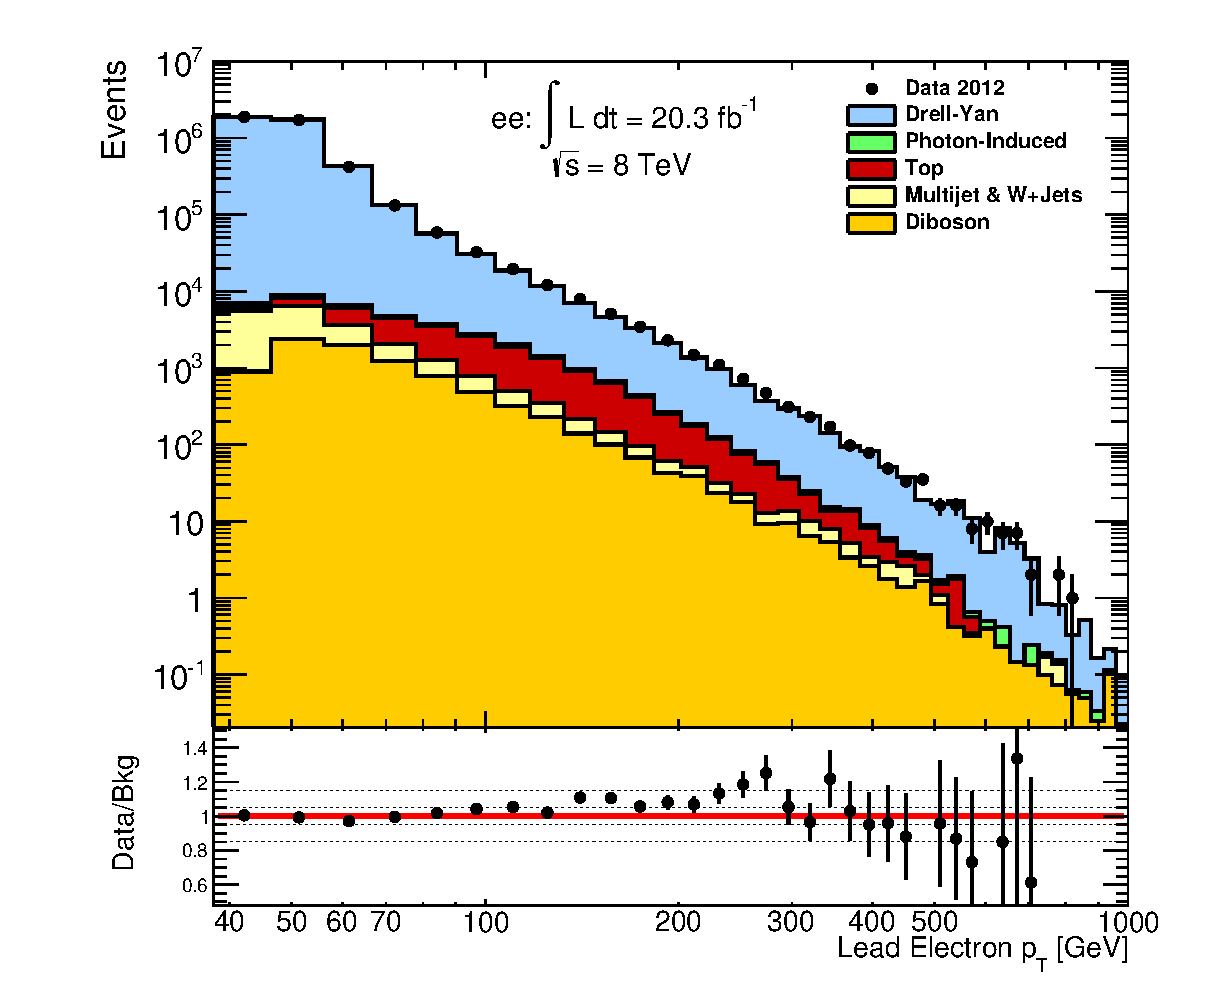
\includegraphics[width=0.49\linewidth]{images/pT_lead.eps}
			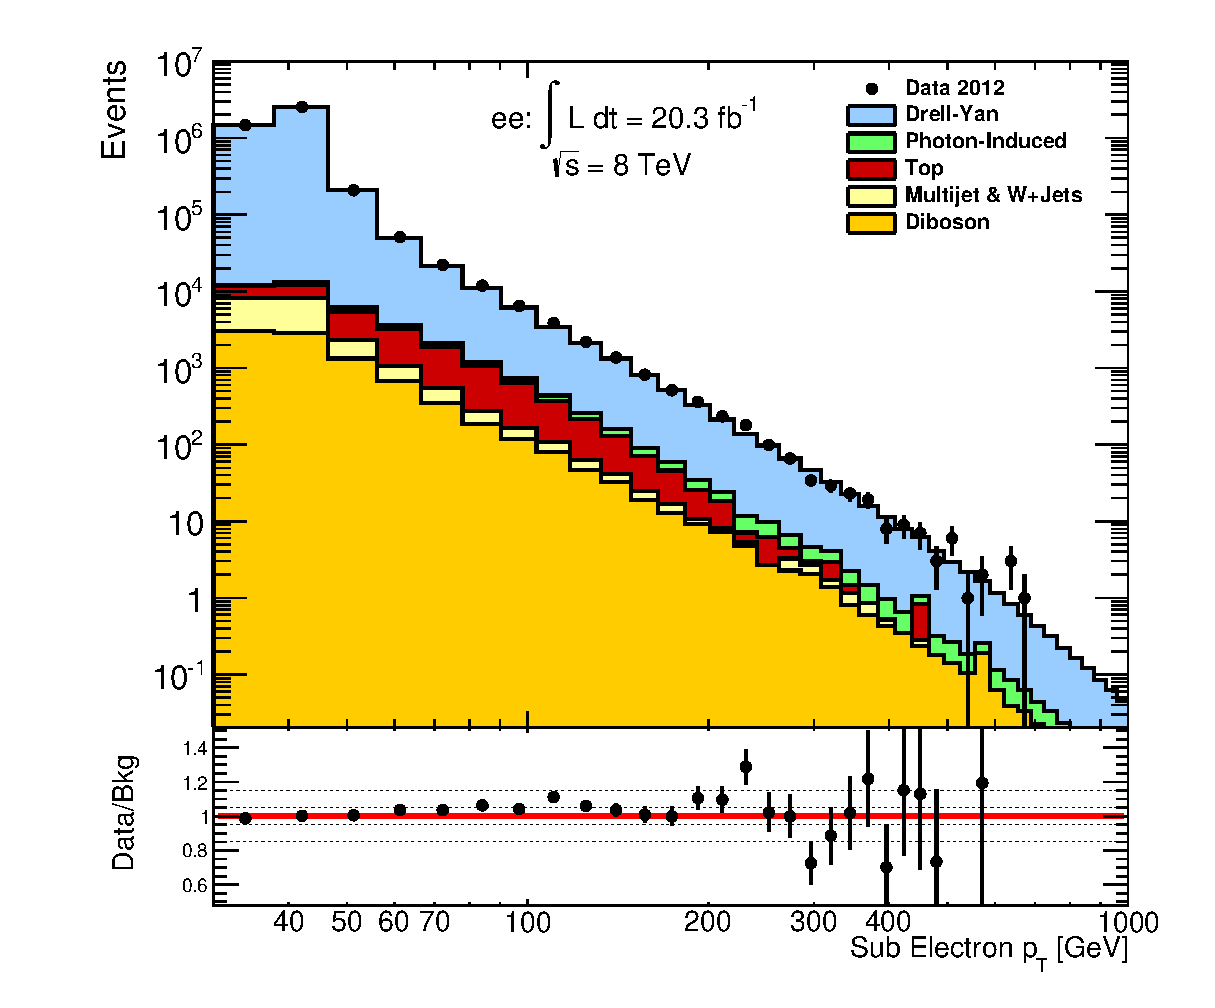
\includegraphics[width=0.49\linewidth]{images/pT_sub.eps}
		\caption{Distribution of p$_{T}$ of the selected highest (left) and second highest (right) p$_{T}$ electrons comparing data to background prediction.}
		\label{fig:app_pt}
	\end{figure}




	\begin{figure}[ht]
		\centering
			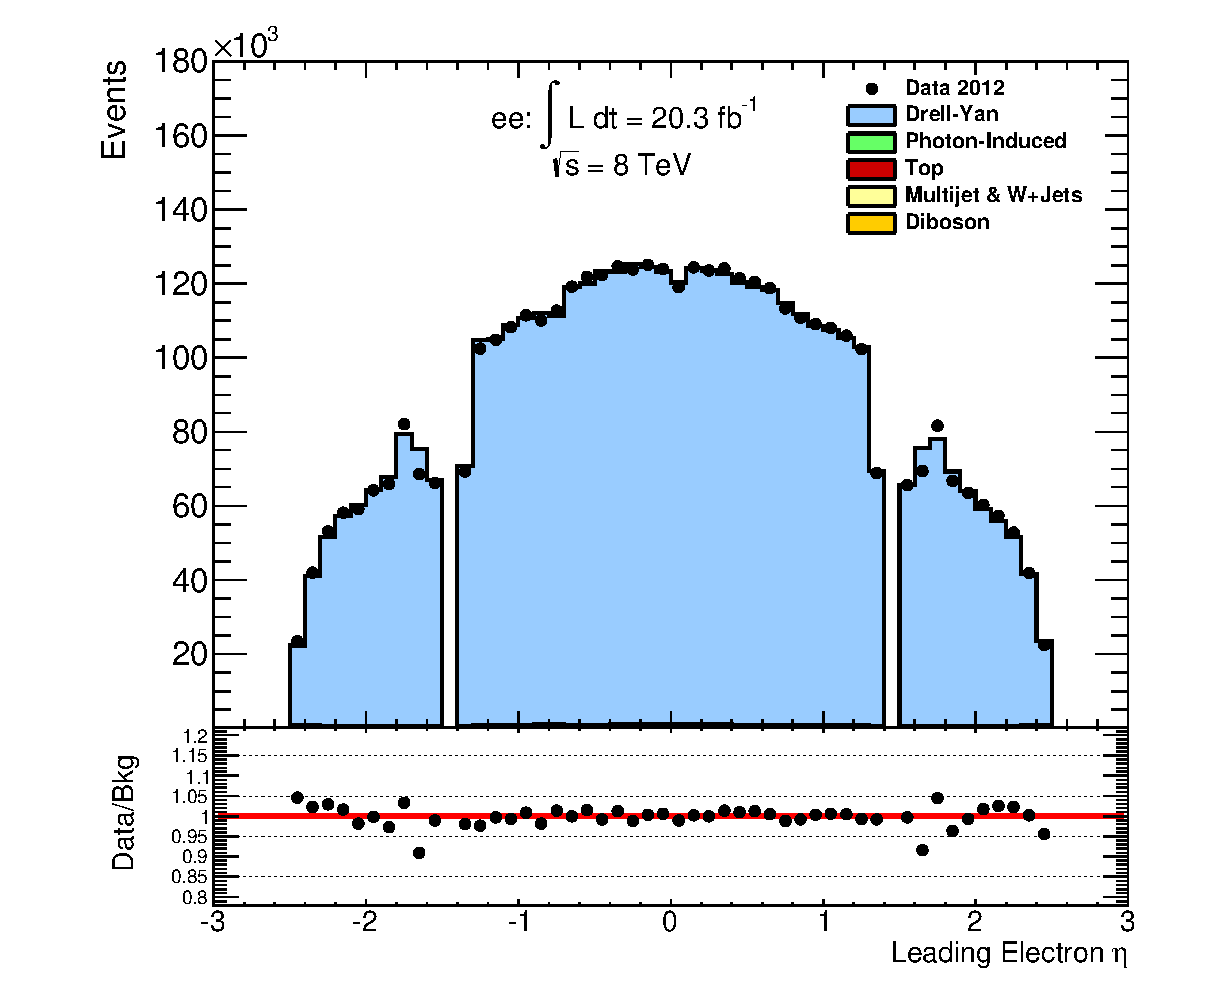
\includegraphics[width=0.49\linewidth]{images/eta_lead.eps}
			\includegraphics[width=0.49\linewidth]{images/eta_sub.eps}
		\caption{Distribution of $\eta$ of the selected highest (left) and second highest (right) p$_{T}$ electrons comparing data to background prediction.}
		\label{fig:app_eta}
	\end{figure}




	% \begin{figure}[ht]
	% 	\centering
	% 		\includegraphics[width=0.9\linewidth]{images/}
	% 	\caption{Distribution of $\phi$ of the selected highest and second highest p$_{T}$ electrons comparing data to background prediction.}
	% 	\label{fig:app_phi}
	% \end{figure}






	\begin{figure}[ht]
		\centering
			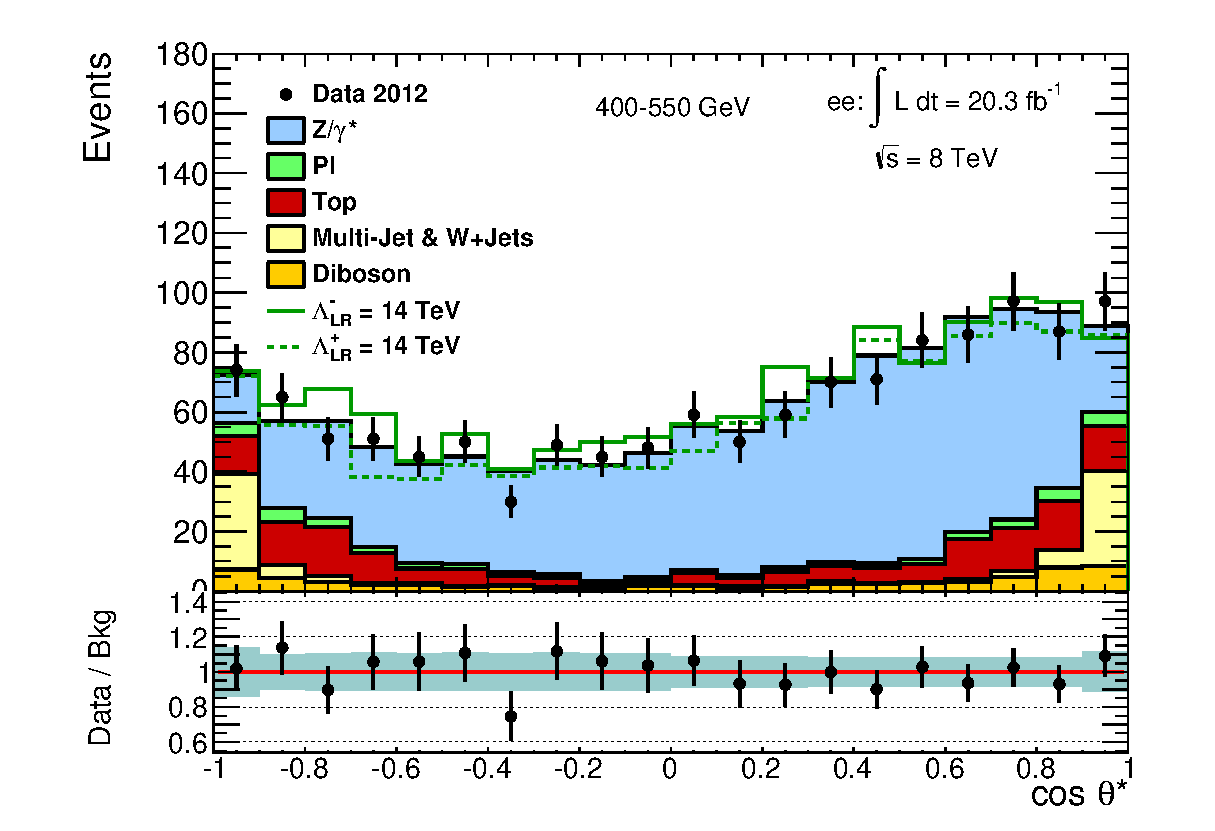
\includegraphics[width=0.9\linewidth]{images/CosThetaStar_bin_1.eps}
		\caption{Plot of $\cos{\theta^{*}}$ comparing background to data in the invariant mass search bin 400-550 GeV with signal overlay.}
		\label{fig:cosTS_1}
	\end{figure}

	\begin{figure}[ht]
		\centering
			\includegraphics[width=0.9\linewidth]{images/CosThetaStar_bin_2.eps}
		\caption{Plot of $\cos{\theta^{*}}$ comparing background to data in the invariant mass search bin 550-800 GeV with signal overlay.}
		\label{fig:cosTS_2}
	\end{figure}


	\begin{figure}[ht]
		\centering
			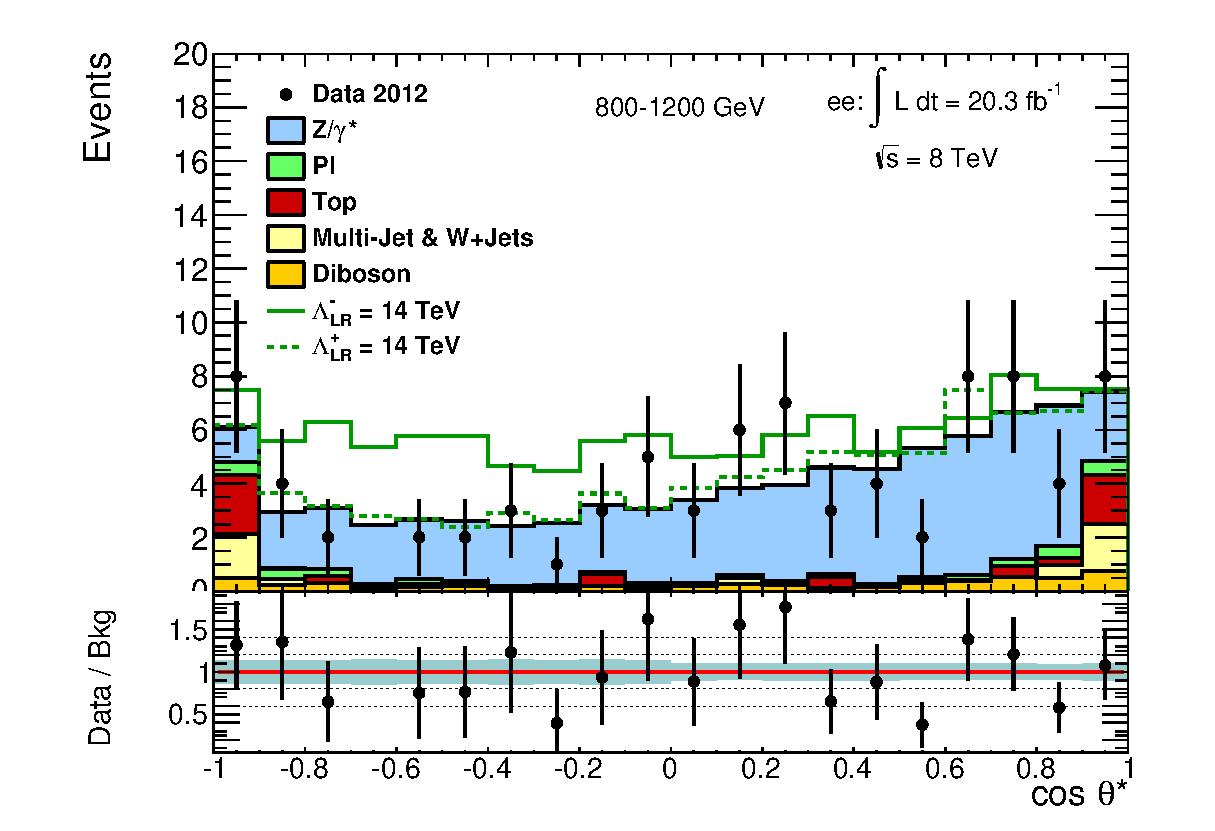
\includegraphics[width=0.9\linewidth]{images/CosThetaStar_bin_3.eps}
		\caption{Plot of $\cos{\theta^{*}}$ comparing background to data in the invariant mass search bin 800-1200 GeV with signal overlay.}
		\label{fig:cosTS_3}
	\end{figure}


	\begin{figure}[ht]
		\centering
			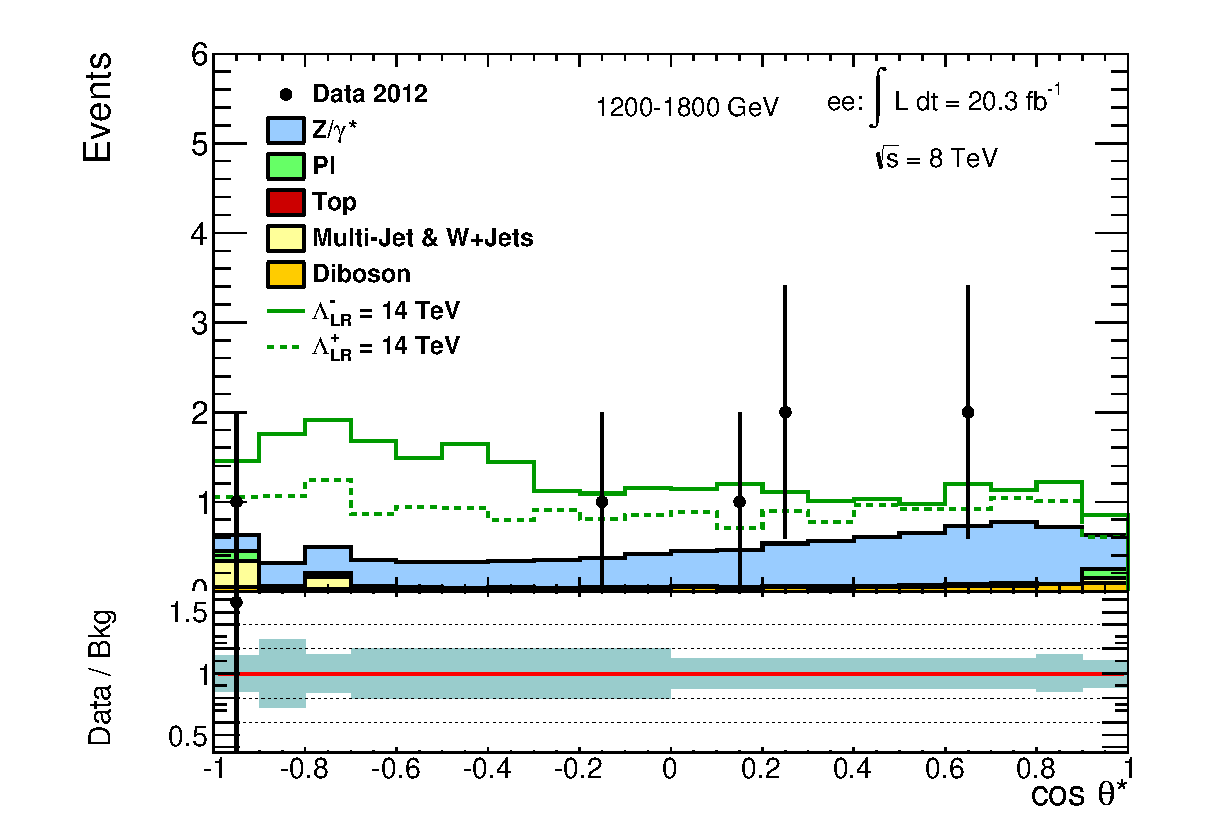
\includegraphics[width=0.9\linewidth]{images/CosThetaStar_bin_4.eps}
		\caption{Plot of $\cos{\theta^{*}}$ comparing background to data in the invariant mass search bin 1200-1800 GeV with signal overlay.}
		\label{fig:cosTS_4}
	\end{figure}


	\begin{figure}[ht]
		\centering
			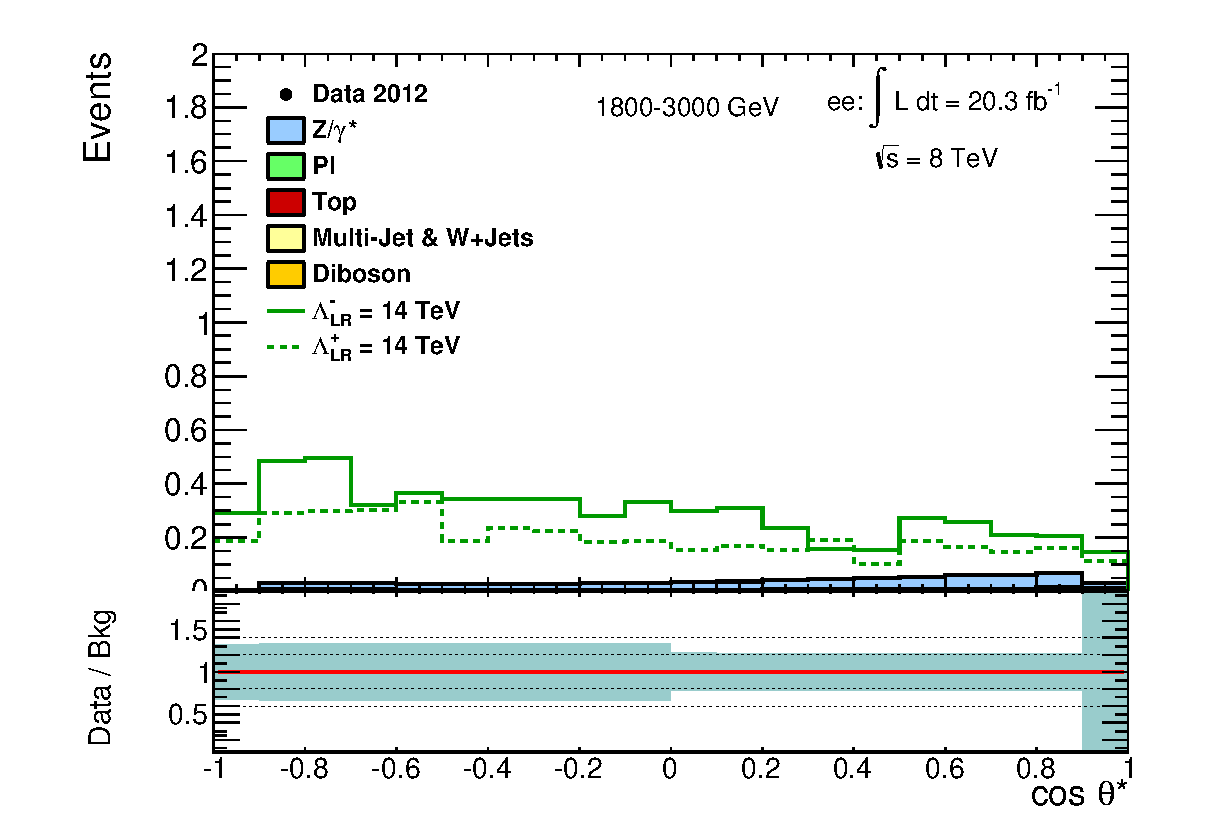
\includegraphics[width=0.49\linewidth]{images/CosThetaStar_bin_5.eps}
			\includegraphics[width=0.49\linewidth]{images/CosThetaStar_bin_6.eps}
		\caption{Plot of $\cos{\theta^{*}}$ comparing background to data in the invariant mass search bins 1800-3000 GeV and 3000-4500 GeV with signal overlay.}
		\label{fig:cosTS_5}
	\end{figure}







	\begin{figure}[ht]
		\centering
			\includegraphics[width=0.49\linewidth]{images/thesis_fits/CI_2D_etaLL_minus_Mass_400-550_GeV_CTS_-1_0.eps}
			\includegraphics[width=0.49\linewidth]{images/thesis_fits/CI_2D_etaLL_minus_Mass_400-550_GeV_CTS_0_1.eps}
			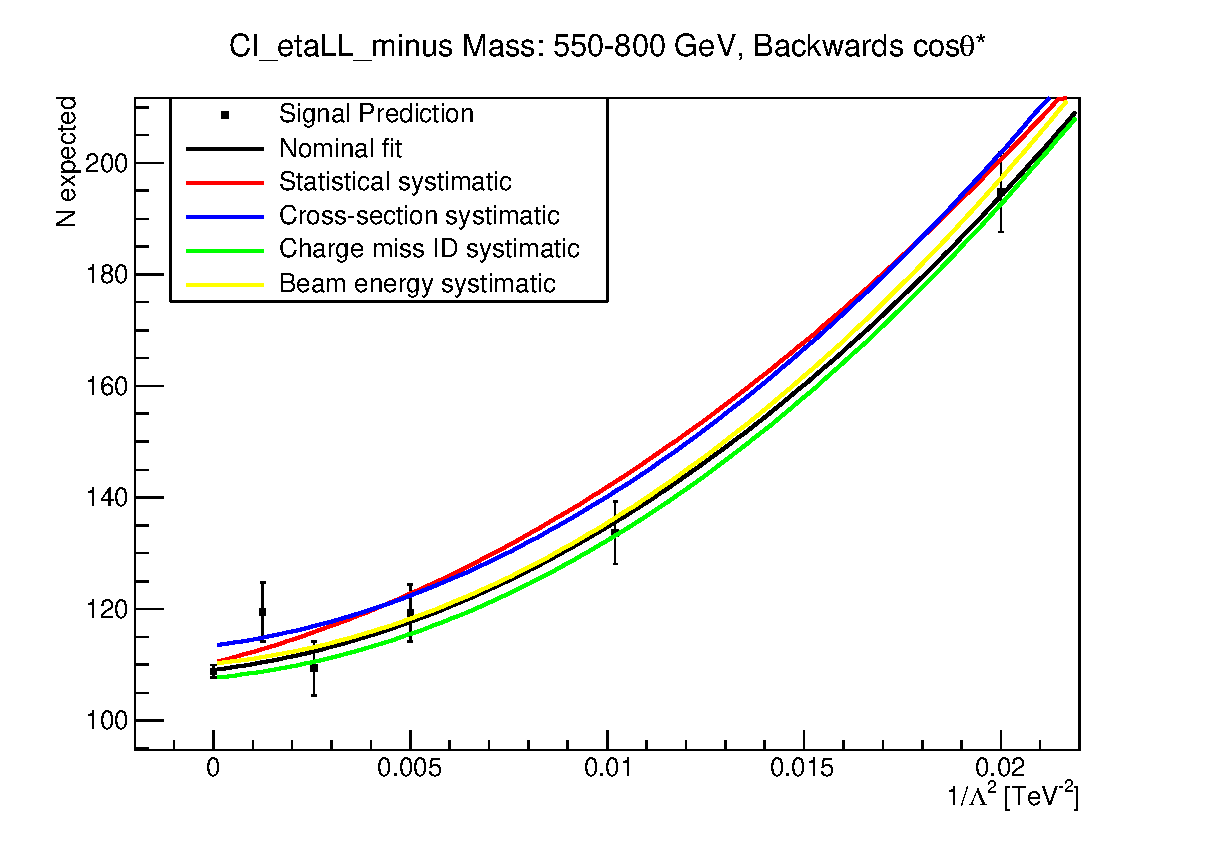
\includegraphics[width=0.49\linewidth]{images/thesis_fits/CI_2D_etaLL_minus_Mass_550-800_GeV_CTS_-1_0.eps}
			\includegraphics[width=0.49\linewidth]{images/thesis_fits/CI_2D_etaLL_minus_Mass_550-800_GeV_CTS_0_1.eps}
			\includegraphics[width=0.49\linewidth]{images/thesis_fits/CI_2D_etaLL_minus_Mass_800-1200_GeV_CTS_-1_0.eps}
			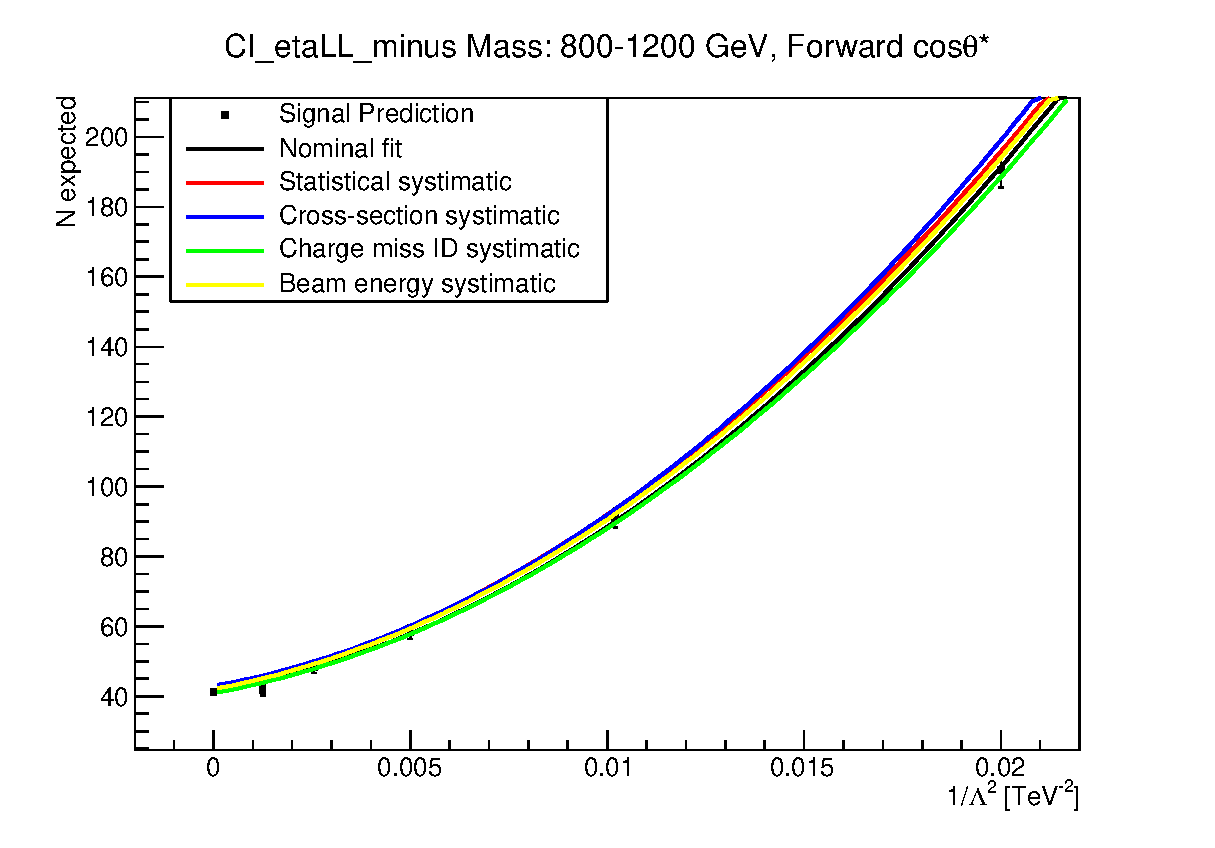
\includegraphics[width=0.49\linewidth]{images/thesis_fits/CI_2D_etaLL_minus_Mass_800-1200_GeV_CTS_0_1.eps}
		\caption{Signal paramaterisations for the LL formalism with constructive interferences for low mass bins}
		\label{fig:parm_LL_m_1}
	\end{figure}

	\begin{figure}[ht]
		\centering
			\includegraphics[width=0.49\linewidth]{images/thesis_fits/CI_2D_etaLL_minus_Mass_1200-1800_GeV_CTS_-1_0.eps}
			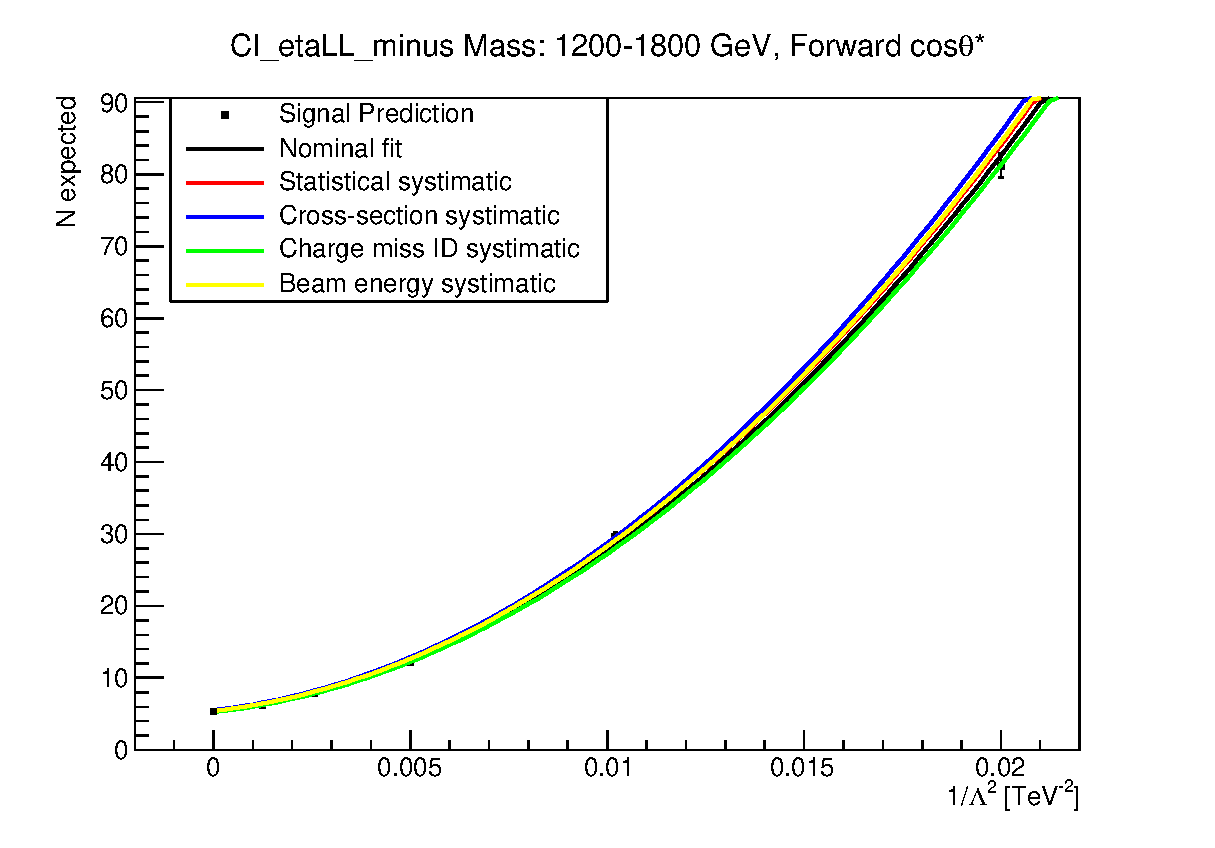
\includegraphics[width=0.49\linewidth]{images/thesis_fits/CI_2D_etaLL_minus_Mass_1200-1800_GeV_CTS_0_1.eps}
			\includegraphics[width=0.49\linewidth]{images/thesis_fits/CI_2D_etaLL_minus_Mass_1800-3000_GeV_CTS_-1_0.eps}
			\includegraphics[width=0.49\linewidth]{images/thesis_fits/CI_2D_etaLL_minus_Mass_1800-3000_GeV_CTS_0_1.eps}
			\includegraphics[width=0.49\linewidth]{images/thesis_fits/CI_2D_etaLL_minus_Mass_3000-4500_GeV_CTS_-1_0.eps}
			\includegraphics[width=0.49\linewidth]{images/thesis_fits/CI_2D_etaLL_minus_Mass_3000-4500_GeV_CTS_0_1.eps}
		\caption{Signal paramaterisations for the LL formalism with constructive interferences for high mass bins}
		\label{fig:parm_LL_m_2}
	\end{figure}


	\begin{figure}[ht]
		\centering
			\includegraphics[width=0.49\linewidth]{images/thesis_fits/CI_2D_etaLL_plus_Mass_400-550_GeV_CTS_-1_0.eps}
			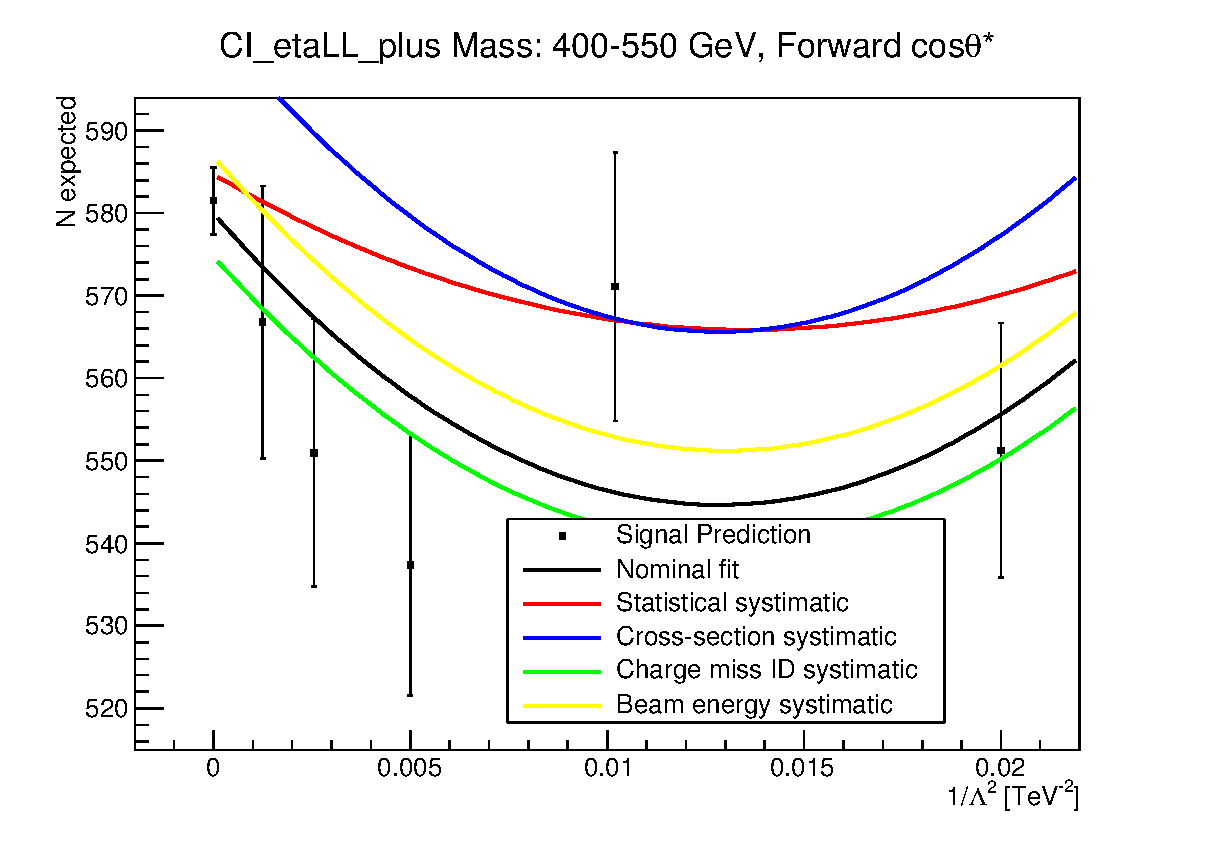
\includegraphics[width=0.49\linewidth]{images/thesis_fits/CI_2D_etaLL_plus_Mass_400-550_GeV_CTS_0_1.eps}
			\includegraphics[width=0.49\linewidth]{images/thesis_fits/CI_2D_etaLL_plus_Mass_550-800_GeV_CTS_-1_0.eps}
			\includegraphics[width=0.49\linewidth]{images/thesis_fits/CI_2D_etaLL_plus_Mass_550-800_GeV_CTS_0_1.eps}
			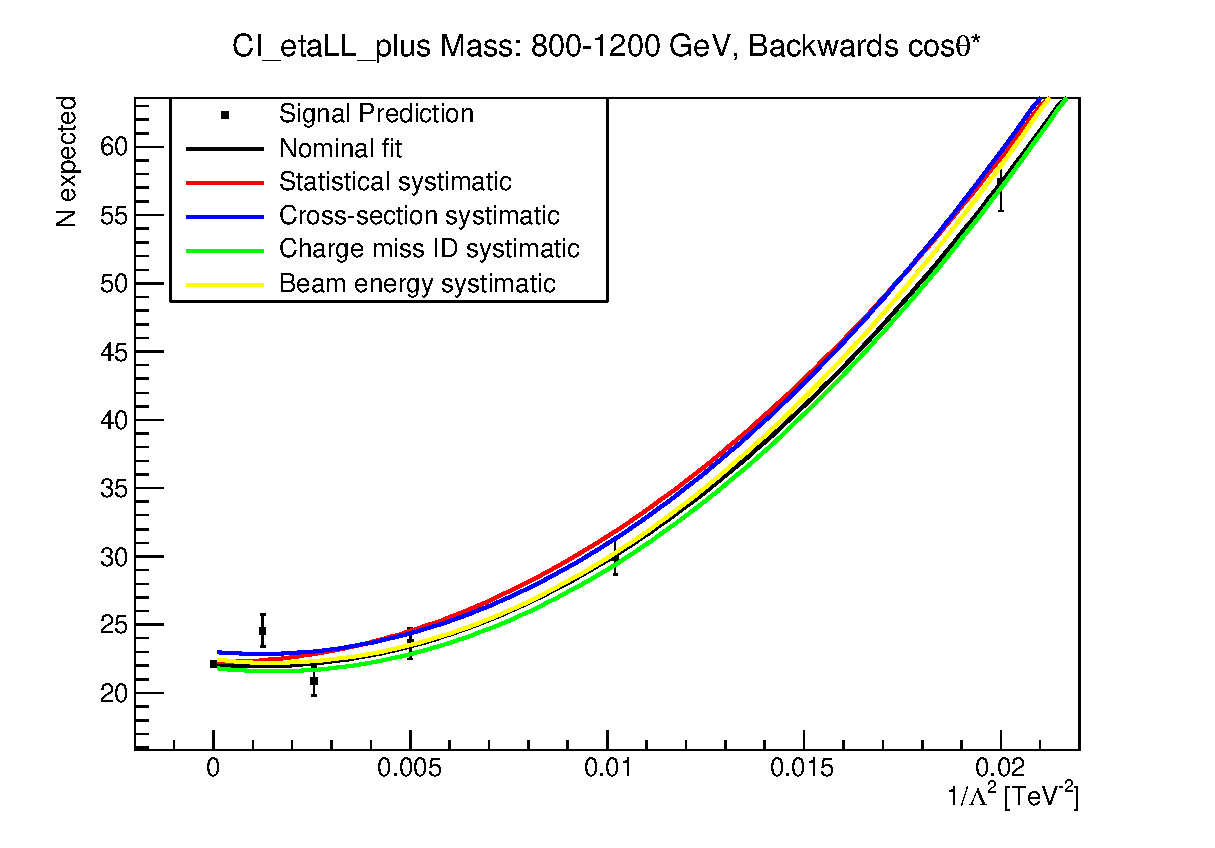
\includegraphics[width=0.49\linewidth]{images/thesis_fits/CI_2D_etaLL_plus_Mass_800-1200_GeV_CTS_-1_0.eps}
			\includegraphics[width=0.49\linewidth]{images/thesis_fits/CI_2D_etaLL_plus_Mass_800-1200_GeV_CTS_0_1.eps}
		\caption{Signal paramaterisations for the LL formalism with destructive interferences for low mass bins}
		\label{fig:parm_LL_p_1}
	\end{figure}

	\begin{figure}[ht]
		\centering
			\includegraphics[width=0.49\linewidth]{images/thesis_fits/CI_2D_etaLL_plus_Mass_1200-1800_GeV_CTS_-1_0.eps}
			\includegraphics[width=0.49\linewidth]{images/thesis_fits/CI_2D_etaLL_plus_Mass_1200-1800_GeV_CTS_0_1.eps}
			\includegraphics[width=0.49\linewidth]{images/thesis_fits/CI_2D_etaLL_plus_Mass_1800-3000_GeV_CTS_-1_0.eps}
			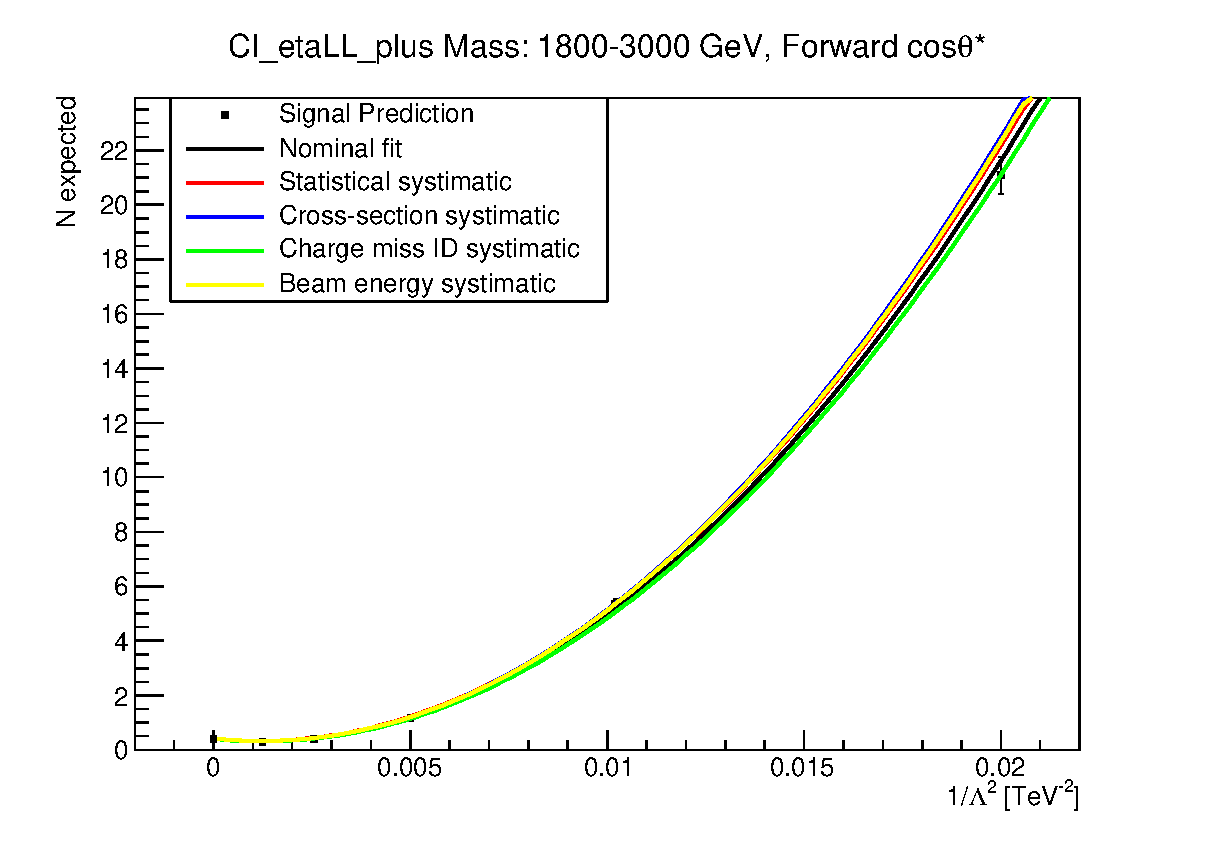
\includegraphics[width=0.49\linewidth]{images/thesis_fits/CI_2D_etaLL_plus_Mass_1800-3000_GeV_CTS_0_1.eps}
			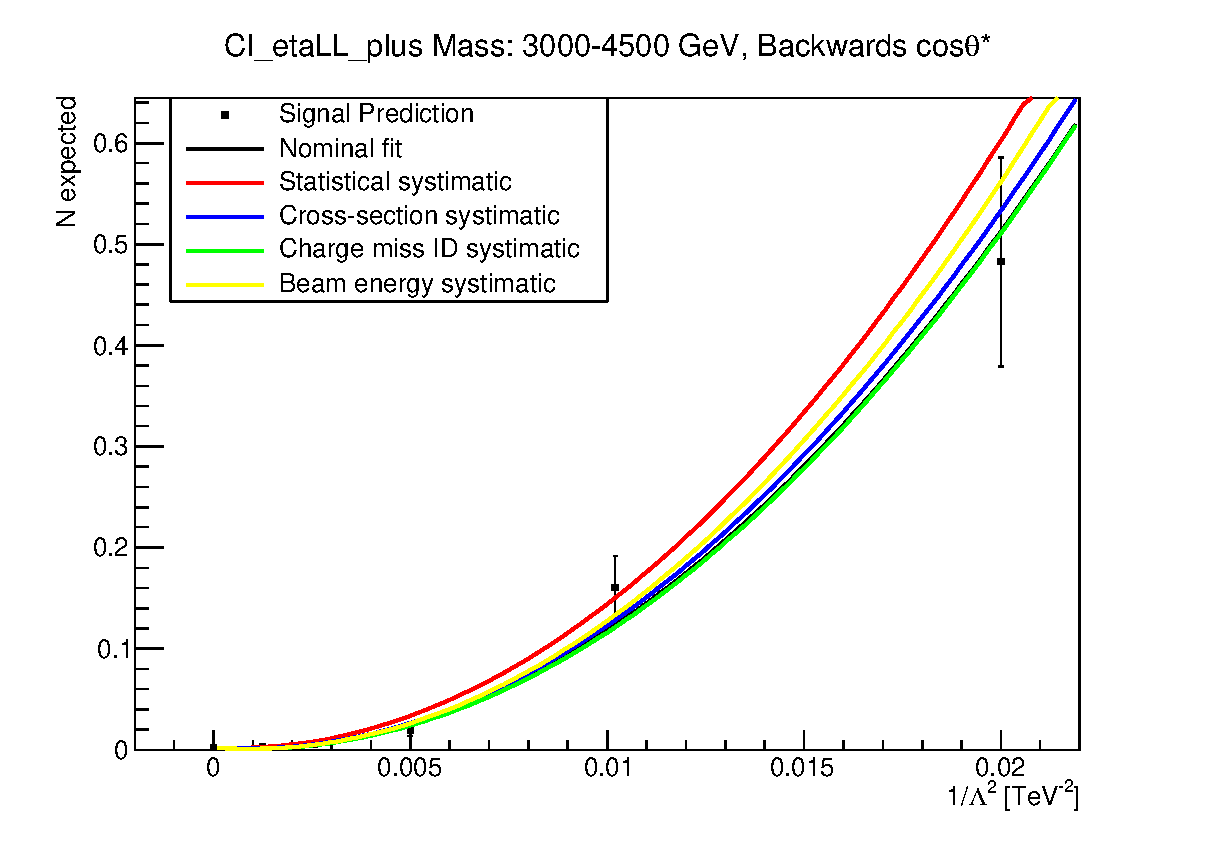
\includegraphics[width=0.49\linewidth]{images/thesis_fits/CI_2D_etaLL_plus_Mass_3000-4500_GeV_CTS_-1_0.eps}
			\includegraphics[width=0.49\linewidth]{images/thesis_fits/CI_2D_etaLL_plus_Mass_3000-4500_GeV_CTS_0_1.eps}
		\caption{Signal paramaterisations for the LL formalism with destructive interferences for high mass bins}
		\label{fig:parm_LL_p_2}
	\end{figure}














	\begin{figure}[ht]
		\centering
			\includegraphics[width=0.49\linewidth]{images/thesis_fits/CI_2D_etaRR_minus_Mass_400-550_GeV_CTS_-1_0.eps}
			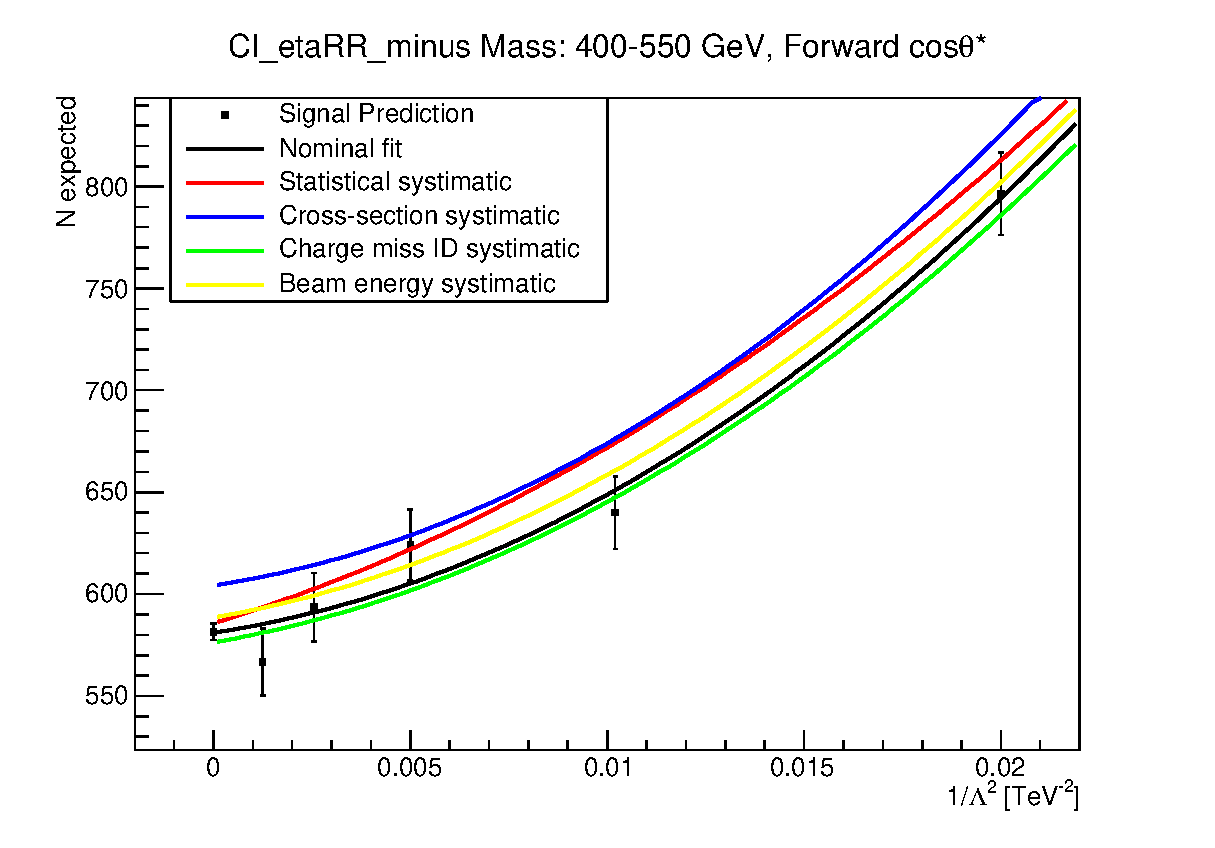
\includegraphics[width=0.49\linewidth]{images/thesis_fits/CI_2D_etaRR_minus_Mass_400-550_GeV_CTS_0_1.eps}
			\includegraphics[width=0.49\linewidth]{images/thesis_fits/CI_2D_etaRR_minus_Mass_550-800_GeV_CTS_-1_0.eps}
			\includegraphics[width=0.49\linewidth]{images/thesis_fits/CI_2D_etaRR_minus_Mass_550-800_GeV_CTS_0_1.eps}
			\includegraphics[width=0.49\linewidth]{images/thesis_fits/CI_2D_etaRR_minus_Mass_800-1200_GeV_CTS_-1_0.eps}
			\includegraphics[width=0.49\linewidth]{images/thesis_fits/CI_2D_etaRR_minus_Mass_800-1200_GeV_CTS_0_1.eps}
		\caption{Signal paramaterisations for the RR formalism with constructive interferences for low mass bins}
		\label{fig:parm_RR_m_1}
	\end{figure}

	\begin{figure}[ht]
		\centering
			\includegraphics[width=0.49\linewidth]{images/thesis_fits/CI_2D_etaRR_minus_Mass_1200-1800_GeV_CTS_-1_0.eps}
			\includegraphics[width=0.49\linewidth]{images/thesis_fits/CI_2D_etaRR_minus_Mass_1200-1800_GeV_CTS_0_1.eps}
			\includegraphics[width=0.49\linewidth]{images/thesis_fits/CI_2D_etaRR_minus_Mass_1800-3000_GeV_CTS_-1_0.eps}
			\includegraphics[width=0.49\linewidth]{images/thesis_fits/CI_2D_etaRR_minus_Mass_1800-3000_GeV_CTS_0_1.eps}
			\includegraphics[width=0.49\linewidth]{images/thesis_fits/CI_2D_etaRR_minus_Mass_3000-4500_GeV_CTS_-1_0.eps}
			\includegraphics[width=0.49\linewidth]{images/thesis_fits/CI_2D_etaRR_minus_Mass_3000-4500_GeV_CTS_0_1.eps}
		\caption{Signal paramaterisations for the RR formalism with constructive interferences for high mass bins}
		\label{fig:parm_RR_m_2}
	\end{figure}


	\begin{figure}[ht]
		\centering
			\includegraphics[width=0.49\linewidth]{images/thesis_fits/CI_2D_etaRR_plus_Mass_400-550_GeV_CTS_-1_0.eps}
			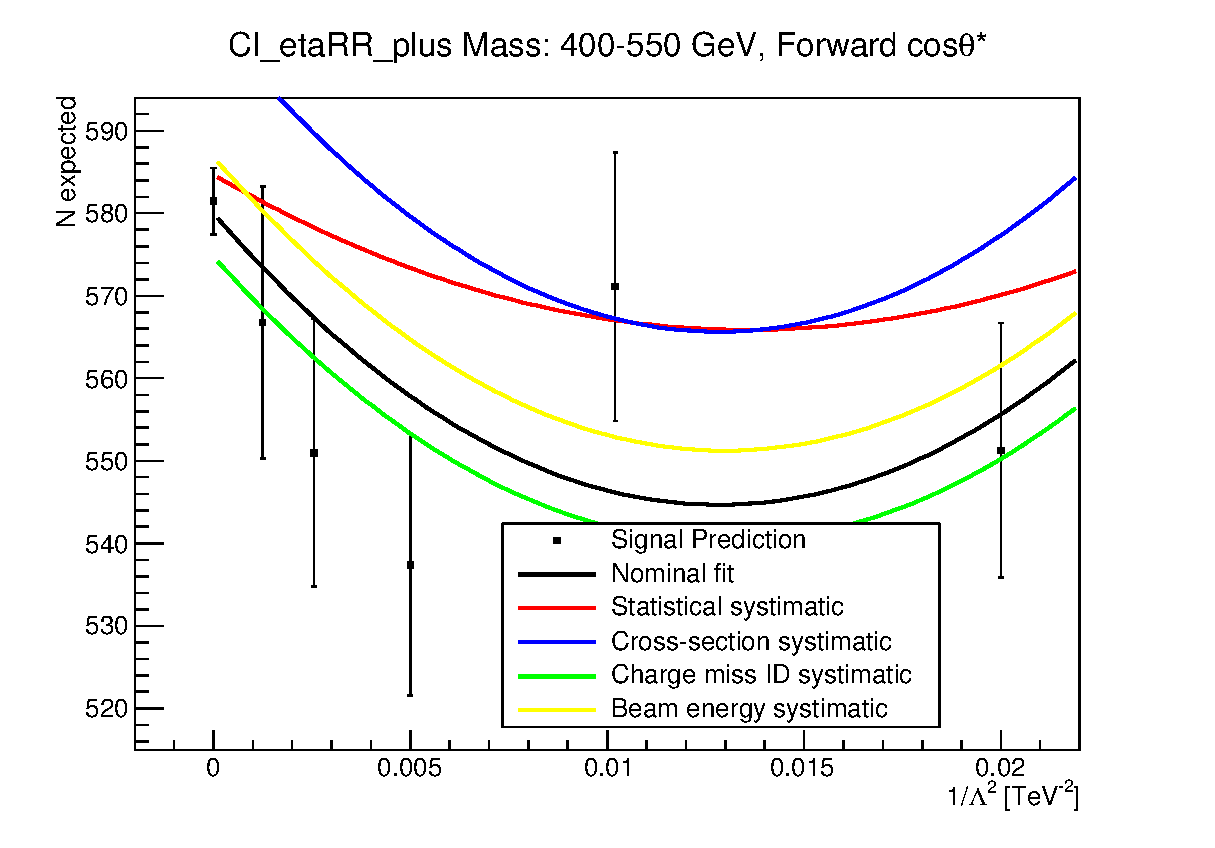
\includegraphics[width=0.49\linewidth]{images/thesis_fits/CI_2D_etaRR_plus_Mass_400-550_GeV_CTS_0_1.eps}
			\includegraphics[width=0.49\linewidth]{images/thesis_fits/CI_2D_etaRR_plus_Mass_550-800_GeV_CTS_-1_0.eps}
			\includegraphics[width=0.49\linewidth]{images/thesis_fits/CI_2D_etaRR_plus_Mass_550-800_GeV_CTS_0_1.eps}
			\includegraphics[width=0.49\linewidth]{images/thesis_fits/CI_2D_etaRR_plus_Mass_800-1200_GeV_CTS_-1_0.eps}
			\includegraphics[width=0.49\linewidth]{images/thesis_fits/CI_2D_etaRR_plus_Mass_800-1200_GeV_CTS_0_1.eps}
		\caption{Signal paramaterisations for the RR formalism with destructive interferences for low mass bins}
		\label{fig:parm_RR_p_1}
	\end{figure}

	\begin{figure}[ht]
		\centering
			\includegraphics[width=0.49\linewidth]{images/thesis_fits/CI_2D_etaRR_plus_Mass_1200-1800_GeV_CTS_-1_0.eps}
			\includegraphics[width=0.49\linewidth]{images/thesis_fits/CI_2D_etaRR_plus_Mass_1200-1800_GeV_CTS_0_1.eps}
			\includegraphics[width=0.49\linewidth]{images/thesis_fits/CI_2D_etaRR_plus_Mass_1800-3000_GeV_CTS_-1_0.eps}
			\includegraphics[width=0.49\linewidth]{images/thesis_fits/CI_2D_etaRR_plus_Mass_1800-3000_GeV_CTS_0_1.eps}
			\includegraphics[width=0.49\linewidth]{images/thesis_fits/CI_2D_etaRR_plus_Mass_3000-4500_GeV_CTS_-1_0.eps}
			\includegraphics[width=0.49\linewidth]{images/thesis_fits/CI_2D_etaRR_plus_Mass_3000-4500_GeV_CTS_0_1.eps}
		\caption{Signal paramaterisations for the RR formalism with destructive interferences for high mass bins}
		\label{fig:parm_RR_p_2}
	\end{figure}
















	\begin{figure}[ht]
		\centering
			\includegraphics[width=0.49\linewidth]{images/thesis_fits/CI_2D_etaLR_minus_Mass_400-550_GeV_CTS_-1_0.eps}
			\includegraphics[width=0.49\linewidth]{images/thesis_fits/CI_2D_etaLR_minus_Mass_400-550_GeV_CTS_0_1.eps}
			\includegraphics[width=0.49\linewidth]{images/thesis_fits/CI_2D_etaLR_minus_Mass_550-800_GeV_CTS_-1_0.eps}
			\includegraphics[width=0.49\linewidth]{images/thesis_fits/CI_2D_etaLR_minus_Mass_550-800_GeV_CTS_0_1.eps}
			\includegraphics[width=0.49\linewidth]{images/thesis_fits/CI_2D_etaLR_minus_Mass_800-1200_GeV_CTS_-1_0.eps}
			\includegraphics[width=0.49\linewidth]{images/thesis_fits/CI_2D_etaLR_minus_Mass_800-1200_GeV_CTS_0_1.eps}
		\caption{Signal paramaterisations for the LR formalism with constructive interferences for low mass bins}
		\label{fig:parm_LR_m_1}
	\end{figure}

	\begin{figure}[ht]
		\centering
			\includegraphics[width=0.49\linewidth]{images/thesis_fits/CI_2D_etaLR_minus_Mass_1200-1800_GeV_CTS_-1_0.eps}
			\includegraphics[width=0.49\linewidth]{images/thesis_fits/CI_2D_etaLR_minus_Mass_1200-1800_GeV_CTS_0_1.eps}
			\includegraphics[width=0.49\linewidth]{images/thesis_fits/CI_2D_etaLR_minus_Mass_1800-3000_GeV_CTS_-1_0.eps}
			\includegraphics[width=0.49\linewidth]{images/thesis_fits/CI_2D_etaLR_minus_Mass_1800-3000_GeV_CTS_0_1.eps}
			\includegraphics[width=0.49\linewidth]{images/thesis_fits/CI_2D_etaLR_minus_Mass_3000-4500_GeV_CTS_-1_0.eps}
			\includegraphics[width=0.49\linewidth]{images/thesis_fits/CI_2D_etaLR_minus_Mass_3000-4500_GeV_CTS_0_1.eps}
		\caption{Signal paramaterisations for the LR formalism with constructive interferences for high mass bins}
		\label{fig:parm_LR_m_2}
	\end{figure}


	\begin{figure}[ht]
		\centering
			\includegraphics[width=0.49\linewidth]{images/thesis_fits/CI_2D_etaLR_plus_Mass_400-550_GeV_CTS_-1_0.eps}
			\includegraphics[width=0.49\linewidth]{images/thesis_fits/CI_2D_etaLR_plus_Mass_400-550_GeV_CTS_0_1.eps}
			\includegraphics[width=0.49\linewidth]{images/thesis_fits/CI_2D_etaLR_plus_Mass_550-800_GeV_CTS_-1_0.eps}
			\includegraphics[width=0.49\linewidth]{images/thesis_fits/CI_2D_etaLR_plus_Mass_550-800_GeV_CTS_0_1.eps}
			\includegraphics[width=0.49\linewidth]{images/thesis_fits/CI_2D_etaLR_plus_Mass_800-1200_GeV_CTS_-1_0.eps}
			\includegraphics[width=0.49\linewidth]{images/thesis_fits/CI_2D_etaLR_plus_Mass_800-1200_GeV_CTS_0_1.eps}
		\caption{Signal paramaterisations for the LR formalism with destructive interferences for low mass bins}
		\label{fig:parm_LR_p_1}
	\end{figure}

	\begin{figure}[ht]
		\centering
			\includegraphics[width=0.49\linewidth]{images/thesis_fits/CI_2D_etaLR_plus_Mass_1200-1800_GeV_CTS_-1_0.eps}
			\includegraphics[width=0.49\linewidth]{images/thesis_fits/CI_2D_etaLR_plus_Mass_1200-1800_GeV_CTS_0_1.eps}
			\includegraphics[width=0.49\linewidth]{images/thesis_fits/CI_2D_etaLR_plus_Mass_1800-3000_GeV_CTS_-1_0.eps}
			\includegraphics[width=0.49\linewidth]{images/thesis_fits/CI_2D_etaLR_plus_Mass_1800-3000_GeV_CTS_0_1.eps}
			\includegraphics[width=0.49\linewidth]{images/thesis_fits/CI_2D_etaLR_plus_Mass_3000-4500_GeV_CTS_-1_0.eps}
			\includegraphics[width=0.49\linewidth]{images/thesis_fits/CI_2D_etaLR_plus_Mass_3000-4500_GeV_CTS_0_1.eps}
		\caption{Signal paramaterisations for the LR formalism with destructive interferences for high mass bins}
		\label{fig:parm_LR_p_2}
	\end{figure}




